\documentclass[11pt]{article}
\usepackage[margin=1in]{geometry}
\usepackage{setspace}
\usepackage{amsmath}
\usepackage{graphicx}
\usepackage{enumitem}
\usepackage{titlesec}
\usepackage{subcaption}
\usepackage[dvipsnames]{xcolor}
\usepackage[colorlinks=true,urlcolor=blue,citecolor=black,linkcolor=black]{hyperref}
\usepackage{multicol}
\usepackage{fancyhdr}
\pagestyle{fancy}
\fancyhf{}
\renewcommand{\headrulewidth}{0pt}
\fancyfoot[L]{\footnotesize ML identification of dynamic interfacial motifs}
\fancyfoot[R]{\footnotesize March 2026 \textbar\ \thepage}
\let\oldbibliography\thebibliography
\renewcommand{\thebibliography}[1]{\oldbibliography{#1}\setlength{\itemsep}{1pt}\setlength{\parsep}{0pt}}

\setstretch{1.0}
\setlist[itemize]{noitemsep, topsep=2pt}
\setlist[enumerate]{noitemsep, topsep=2pt}

\titleformat{\section}{\large\bfseries}{\thesection.}{0.5em}{}
\titlespacing*{\section}{0pt}{4pt}{2pt}
\titleformat{\subsection}{\normalsize\bfseries}{\thesubsection}{0.5em}{}
\titlespacing*{\subsection}{0pt}{3pt}{1pt}

\begin{document}

\begin{center}
{\Large \textbf{Machine-Learning Identification of Dynamic Interfacial Motifs Governing Plastic Response}}\\
\vspace{0.3em}
{\normalsize PI: Dr.\ Menahem Krief \quad Student: Dolev Ronen}\\
\vspace{0.3em}
\end{center}

\section*{Background, research question, and innovation}

Dislocations carry plastic deformation by moving collectively along slip planes \cite{Cordero2016}.
In single crystals the Dislocation Extraction Algorithm (DXA) tracks them reliably \cite{Stukowski2012}, but in polycrystals much of the plastic activity occurs at grain boundaries (GBs), where dislocations pile up, get absorbed, or transmit \cite{Piao2022,Liu2020,DGI2025}.
These processes control Hall-Petch strengthening, back stress, and ductility \cite{Cordero2016,Gao2022,LeBauschinger2018}.
Continuum models such as Le's thermodynamic dislocation theory parametrise the GB through impedance-like boundary conditions (impermeable, transfer-permitting, or absorbing/re-emitting) and predict different work hardening for each case \cite{Piao2022,LeBauschinger2018}, but the parameters remain phenomenological because GB activity has not been directly measured.
In prior work, the PI and Co-I mapped local elastic moduli in nanocrystalline Cu and Ta, revealing mechanical heterogeneity concentrated at GBs \cite{Krief2024}; that study established the per-atom extraction methodology on which this proposal builds.
DXA fails inside high-angle GBs because Burgers circuits do not close in the disordered core \cite{Stukowski2012}, and Interfacial Line Defect Analysis (ILDA) \cite{Deka2023} still requires bicrystal reference states.
The problem is acute in nanocrystalline metals where GB deformation dominates below ${\sim}10$\,nm grain size \cite{Gupta2020}; using Common Motion Grouping (CMG), Dimanstein Firman \emph{et al.}\ showed that most mobile dislocations reside \emph{within} the GB, invisible to DXA \cite{Firman2024}.

Several independent results show that GB plasticity is structured: thermally activated point-defect avalanches spanning 10-20\,nm along metallic GBs \cite{Chesser2022}, learned softness fields predicting rearrangement barriers \cite{Sharp2018}, and disconnection-controlled GB response observed experimentally \cite{Gautier2025}.
Combined with CMG evidence of dislocation-like correlated motion inside GBs \cite{Firman2024}, this raises a central question: \emph{can we identify the dynamic motifs that carry plasticity inside the GB?}

\textbf{Innovation.} We propose the first transfer-learning approach that trains on DXA-labelled dislocations in the grain interior and applies the learned representation to the GB core where DXA fails. Unlike DXA (geometric), CMG (correlational), or softness (scalar), a convolutional neural network (CNN) can learn a transferable representation from both structural and kinematic features. The longer-term aim is to extract constitutive parameters (absorption rates, impedance, transmission probabilities) for mesoscale models \cite{Bertin2024,Kedharnath2024,Piao2022,LeBauschinger2018}.

\section*{Research hypothesis}

The same fingerprint that defines a bulk dislocation, correlated atomic motion along a slip direction, persists inside the disordered GB but has not been classified.
We hypothesise that GB plasticity takes the form of \emph{dynamic interfacial motifs}: recurring patterns in local structure (stress, energy) and motion (correlated velocities) that resemble lattice dislocations. A model trained where DXA labels exist should generalise to the GB core.
Such motifs would provide a physically interpretable intermediate representation: richer than a scalar softness field, yet tractable enough to parameterise mesoscale plasticity models.

\textbf{Testable targets:}
\begin{enumerate}
    \item \textbf{Detection:} CNN precision and recall on held-out grain-interior frames competitive with DXA.
    \item \textbf{Transfer:} coherent activity maps in the GB core consistent with known slip-transfer events on at least one high-angle boundary.
    \item \textbf{Mechanical correlation:} CNN-derived GB activity metrics correlate with flow stress and reverse yield beyond bulk dislocation density alone.
\end{enumerate}

\section*{Proposed use of artificial intelligence}

The pipeline has two stages (Fig.~\ref{fig:pipeline}).

\textbf{Stage 1: supervised training in the grain interior.}
DXA provides ground-truth dislocation labels (locations, Burgers vectors, line characters). Per-atom stress, velocity, and potential energy are mapped onto a 3D voxel grid, extending Noh and Chew's 2D pixelation \cite{Noh2024}. A CNN is trained to reproduce the DXA map on that grid, with voxel size chosen to resolve individual partial dislocations (${\sim}5$\,\AA).
The gridded field representation naturally suits convolutional architectures, and Noh and Chew have shown that CNNs can learn the mechanical signature of a dislocation near an interface. Velocity fields are essential: they capture correlated motion and distinguish active dislocations from static disorder. The loss is the per-voxel discrepancy between CNN output and DXA label.

\textbf{Stage 2: transfer to the GB core.}
The trained CNN is applied inside the disordered GB where DXA cannot operate, producing an activity map that extends continuously from the grain interior (where it agrees with DXA) into the GB core (where it provides new information).
Evaluation uses held-out DXA labels in the interior (precision, recall, F1) and hand-curated GB frames.
We test whether CNN-derived GB activity metrics (active area fraction, event count) correlate with macroscopic observables (flow stress, reverse yield, hysteresis area) beyond what bulk dislocation density alone explains.

\begin{figure}[ht]
\centering
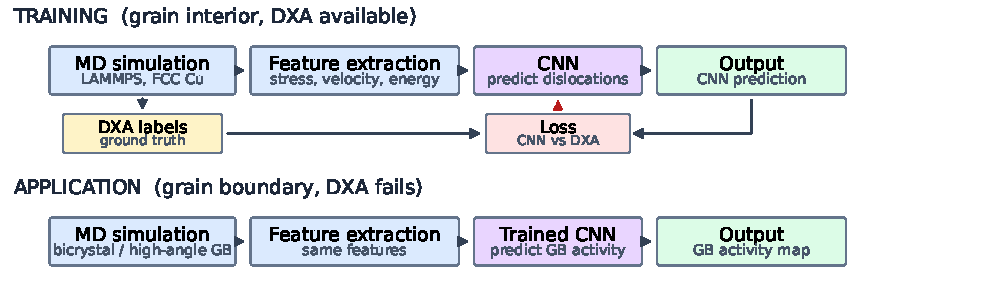
\includegraphics[width=\textwidth]{graphs/pipeline.pdf}
\caption{\small Training (top) and application (bottom) pipeline.}
\label{fig:pipeline}
\end{figure}

\textbf{Risk mitigation.}
Domain shift is mitigated by staged training: bulk single crystals first, then the near-GB zone of low-angle boundaries, then high-angle GBs.
Velocity features separate dislocation activity from static GB disorder; spatial post-processing enforces line connectivity.

\section*{Data types to be processed and expected scope}

All data are classical MD trajectories (LAMMPS, EAM, FCC Cu), building on the group's simulation pipeline \cite{Krief2021,Krief2024}.
Cu with an EAM potential is a well-characterised model FCC system with established dislocation mobilities and stacking fault energies, making it ideal for validating the method before extending to more complex alloys.
Bulk runs supply DXA-labelled training data; bicrystal runs (low- to high-angle tilt, selected asymmetric boundaries) provide transfer targets.
Per-atom stress, velocity, and energy are dumped at 0.5\,ps resolution.
Monotonic and tension/compression reversal protocols connect defect evolution to Bauschinger observables \cite{Gao2022}; the DGI dataset \cite{DGI2025} is an additional test set.
MD strain rates ($10^{8}$-$10^{10}\,\mathrm{s^{-1}}$) amplify interfacial modes, making GBs a strong source of plastic events in simulation.

\begin{center}
\small
\begin{tabular}{|l|c|c|l|}
\hline
\textbf{Run type} & \textbf{Runs} & \textbf{Atoms} & \textbf{Purpose} \\
\hline
Bulk single-crystal & 6 & $2\!\times\!10^{5}$ & DXA-supervised training \\
Bicrystal (6 GBs $\times$ 2 protocols) & 12 & $3\!\times\!10^{5}$ & Transfer \& reversal \\
Nanocrystalline & 2 & $10^{6}$ & Polycrystal stress test \\
\hline
\multicolumn{4}{|l|}{Total: ${\sim}\!20$ runs, ${\sim}\!300$\,GB data, ${\sim}\!300$ core-h MD (CPU cluster, ${\leq}\!2048$ cores) $+$ ${\sim}\!100$ GPU-h (CNN)} \\
\hline
\end{tabular}
\end{center}

\noindent Resources provided through the PI's \href{http://icpl.huji.ac.il}{ICPL} membership; no compute budget requested.

\section*{Project timeline (12 months)}

\noindent\resizebox{\textwidth}{!}{%
\small
\begin{tabular}{|c|c|c|c|c|}
\hline
\textbf{M1-3} & \textbf{M4-6} & \textbf{M7-9} & \textbf{M10-11} & \textbf{M12} \\
\hline
MD, DXA, features & CNN training & GB transfer, ILDA & Reversal, correlation & Manuscript, PhD prop.\ \\
\hline
\end{tabular}}

\section*{Applicants and principal investigator}
All members are from the Racah Institute of Physics, The Hebrew University of Jerusalem.
\textbf{PI:} Dr.\ Menahem Krief (computational materials science, ML for atomistic simulations). Krief developed methods for local elastic constants from MD \cite{Krief2021} and mapped elastic heterogeneity across nanocrystalline GBs \cite{Krief2024}; the same feature-extraction infrastructure and Cu/EAM pipeline are reused here.
\textbf{Co-I:} Prof.\ Yinon Ashkenazy (MD methodology, nanocrystalline mechanics; developer of CMG \cite{Firman2024}).
\textbf{M.Sc.\ student:} Dolev Ronen, completing his M.Sc.\ in Physics.
This seed project serves a dual purpose: establishing whether the proposed transfer-learning methodology is viable, and equipping Dolev with the MD, data-processing, and ML skills needed for doctoral research. A successful outcome will form the basis of a PhD proposal.

\section*{Requested budget and justification}
We request \textbf{100,000~NIS} for 12 months:
\begin{itemize}
    \item \textbf{Scholarship}, Dolev Ronen (M.Sc.): \textbf{84,000~NIS} (12 $\times$ 7,000~NIS/month).
    \item \textbf{Travel}: \textbf{16,000~NIS} for conference presentation and US collaboration visits.
\end{itemize}
GPU time provided by \href{http://icpl.huji.ac.il}{ICPL}; no compute budget requested.

\section*{Future plans}

This project is a 12-month feasibility study. We aim to deliver: a documented MD-to-ML pipeline, trained CNN models for Cu bicrystals, a precision/recall benchmark against DXA, and proof-of-concept GB activity maps.
These results will support a \textbf{PhD proposal} (ISF or equivalent) for Dolev Ronen, structured as a three-year programme around three extensions:
(i)~extracting GB constitutive parameters (absorption rates, transmission probabilities, impedance) for discrete dislocation dynamics (DDD) and continuum models \cite{Piao2022,LeBauschinger2018,Bertin2024};
(ii)~transferring to BCC metals (W, Ta, Fe) where dislocation core structure, slip geometry, and GB chemistry differ qualitatively from FCC;
and (iii)~experimental validation via EBSD and in-situ TEM \cite{Gautier2025}.
The ultimate test is whether learned parameters predict macroscopic observables (back stress, Bauschinger asymmetry, Hall-Petch scaling) better than current empirical fits.
The project will also build ML methodology and simulation infrastructure within the group for future computational materials science work.

{\footnotesize
\begin{multicols}{2}
\bibliographystyle{unsrt}
\bibliography{references}
\end{multicols}
}

\end{document}
